% Generated from arXiv:2510.11766; see tools/build_source_compendium.py.
\section{Calculation laboratory V: Radial monodromy from oscillator to Coulomb}
\label{lab:2510_11766}

\calculationroute
  {Exact WKB on a regular contour, Frobenius indices at the origin, closed-cycle periods, and the Langer transformation.}
  {The radial Riccati problem, oscillator and Coulomb benchmarks, the exponential map, optimized perturbation theory, anharmonic and Cornell/Yukawa examples, and the open-path/closed-cycle theorem.}
  {Derive radial quantization from both open paths and closed cycles, then reproduce the oscillator, Coulomb, Cornell, and Yukawa checks.}

This Laboratory reconstructs the calculation underlying
Ref.~\cite{Morikawa:2025ezl}.  The regular-contour exact-WKB recursion is not
repeated.  The starting point is the new datum introduced by a radial problem:
the singular endpoint and its monodromy.

\begin{comment}
\subsection{Exact WKB analysis for general radial Schr\"odinger equation}\label{src:2510_11766:sec:resurgence-wkb}
\subsubsection{Introducing WKB ansatz}
We shall consider a $3$-dimensional Schr\"odinger equation,
\begin{align}
    \left[ -\frac{\hbar^2}{2}\nabla^2 + V(\bm{x}) \right] \psi(\bm{x})
    = E \psi(\bm{x}) .
\end{align}
If we analyze this differential equation and quasi-stationary states in a non-perturbative manner, for instance in resurgence theory, the coordinate $x$ is complexified, and the crucial technique is given by the complex analysis and the resummation of higher-order/singular perturbations.
A well-established framework for resurgence theory is provided by the exact WKB method, which is applicable to differential equations with respect to one variable. Then, in general, we now focus on the radial Schr\"odinger equation with an angular momentum~$l$
\begin{align}
    \left[-\frac{\hbar^2}{2}\frac{\rmd^2}{\rmd r^2} + V(r) + \frac{\hbar^2}{2}\frac{l(l+1)}{r^2} - E\right] \varphi_l(r) = 0 ,
\end{align}
or
\begin{align}
    \left[-\frac{\rmd^2}{\rmd r^2} + \hbar^{-2}Q(r)\right] \varphi_l(r) = 0, \qquad
    Q(r) = \frac{1}{r} Q_0(r) + \frac{\hbar^2}{r^2} Q_2(r),
\end{align}
where
\begin{align}
        Q_0(r) \equiv 2r\left[V(r) - E\right], \qquad Q_2(r) \equiv Q_2 = l(l+1) .
\end{align}
Let us introduce the WKB ansatz of the radial Schr\"odinger equation as a formal power series,
\begin{align}
    \varphi_l(r,\hbar) &= \rme^{\int^r \rmd r'\, S(r',\hbar)} ,&
    S(r,\hbar) &= \sum_{i=-1}^{\infty}\hbar^{i} S_{i}(r) .
\end{align}
Substituting $S(r,\hbar)$ into the radial Schr\"odinger equation, we see the Riccati equation
\begin{align}
    S^2 + \frac{\rmd S}{\rmd r} = \hbar^{-2} Q .
    \label{src:2510_11766:eq:riccati_eq}
\end{align}
The recursive equation of $S_i$ for each power of~$\hbar$ holds as
\begin{align}
    \hbar^{-2}&:S_{-1}^2 = \frac{Q_0(r)}{r} ,
    \label{src:2510_11766:eq:recursive_eq_1}\\
    \hbar^{-1}&:2S_{-1}S_{0} + \frac{\rmd S_{-1}}{\rmd r} = 0 ,
    \label{src:2510_11766:eq:recursive_eq_2}\\
    \hbar^{0}&:2S_{-1}S_{1} + S_{0}^2 + \frac{\rmd S_{0}}{\rmd r} = \frac{Q_2}{r^2} ,
    \label{src:2510_11766:eq:recursive_eq_3}\\
    \hbar^{i-1}&:2S_{-1}S_{i} + \sum_{j=0}^{i-1} S_{j}S_{i-j}
    + \frac{\rmd S_{i-1}}{\rmd r} = 0 \qquad i\geq2.
    \label{src:2510_11766:eq:recursive_eq}
\end{align}
We have the two leading-order solutions of~Eq.~\eqref{src:2510_11766:eq:recursive_eq_1}
\begin{align}
    S_{-1}(r) = S_{-1}^{\pm}(r) \equiv \pm \sqrt{\frac{Q_0(r)}{r}} ,
\end{align}
and then can determine all higher-order terms~$S_i$ with $i\geq0$ so that
\begin{align}
    S^{\pm}(r;\hbar) = \sum_{i=-1}^{\infty} \hbar^i S_i^{\pm}(r) .
\end{align}
From Eqs.~\eqref{src:2510_11766:eq:recursive_eq_1}--\eqref{src:2510_11766:eq:recursive_eq}, $S_i^{-}=(-1)^i S_i^{+}$ holds for $i\geq-1$. If there exists $Q_1(r)$ as the $O(\hbar)$ term in $Q(r)$, this relation breaks down. Hence, we can rewrite $S^{\pm}$ by
\begin{align}
    S^{\pm}(r;\hbar)&=\pm \vsub{S}{odd}(r;\hbar) + \vsub{S}{even}(r;\hbar),
    \\
    \vsub{S}{odd}(r;\hbar)&\equiv\sum_{i\geq0}\hbar^{2i-1} S_{2i-1}(r), \quad \vsub{S}{even}(r;\hbar)\equiv\sum_{i\geq0}\hbar^{2i} S_{2i}(r) .
\end{align}
\begin{prop*}
    \begin{align}
        \vsub{S}{even}
        = - \frac{1}{2} \frac{1}{\vsub{S}{odd}}
        \frac{\rmd}{\rmd r} \vsub{S}{odd}
        = - \frac{1}{2}\frac{\rmd}{\rmd r} \ln \vsub{S}{odd}
    \end{align}    
\end{prop*}
The above proposition holds from the fact that the Riccati equation~\eqref{src:2510_11766:eq:riccati_eq} becomes
\begin{align}
    2 \vsub{S}{odd}\vsub{S}{even} + \frac{\rmd}{\rmd r} \vsub{S}{odd} = 0 .
\end{align}
We can rewrite $\vsub{S}{even}$ by~$\vsub{S}{odd}$ in the WKB wave function, and then we obtain
\begin{align}
    \varphi_l(r,\hbar)^{\pm} = \frac{1}{\sqrt{\vsub{S}{odd}(r;\hbar)}}
    \rme^{\pm\int^r \rmd r'\, \vsub{S}{odd}(r';\hbar)}.
\end{align}
\subsubsection{Borel resummation and Stokes geometry}
The power series of the wave function
\begin{align}
    \varphi_l(r,\hbar)^{\pm}
    = \rme^{\pm\hbar^{-1}\int^r \rmd r'\sqrt{Q_0(r')/r'}}
    \sum_{n\geq0} \varphi_{ln}^{\pm}(r) \hbar^{n+1/2}
\end{align}
is an asymptotic series and not necessarily convergent.
Now, we define the Borel transform by
\begin{align}
    \mathcal{B}[\varphi_l^{\pm}](u)\equiv\sum_{n\geq0} \frac{\varphi_{ln}^{\pm}(r)}{\Gamma(n+1/2)} (u\pm u_0)^{n-1/2} ,
\end{align}
where $u_0 = \int^{r} \rmd r'\sqrt{Q_0(r')/r'}$.
The Borel sum is given by
\begin{align}
    \Psi_l(r,\hbar)^{\pm}
    &\equiv \int_{\mp u_0}^\infty \rmd u\, \rme^{-u/\hbar}
    \mathcal{B}[\varphi_l^{\pm}](u) .
\end{align}
Here $\varphi$ is redefined as~$\Psi$.
For divergent series, the Borel transform itself may develop a pole singularity (Borel singularity). If there exists no singular point on the integration path over~$u$, the series is Borel summable. The Borel summable region in the complex $r$-plane is determined as follows:
We introduce turning points as
\begin{align}
    \exists a,\, \left.\frac{Q_0(r)}{r}\right|_{r=a} = 0 ,
\end{align}
or an endpoint $a=0$ in the case that the simple pole in the potential is at the origin.
A Stokes curve is defined by
\begin{align}
    \im \hbar^{-1}\int_a^r \rmd r' \sqrt{\frac{Q_0(r')}{r'}} = 0. \label{src:2510_11766:eq:stokes_curve}
\end{align}
\begin{thm*}
If ``$a$'' is a turning point, by using the Airy equation, there are three Stokes curves extending from~``$a$''; if ``$a$'' is a simple pole, one Stokes curve is derived by the Laurent expansion.
\end{thm*}
When an integration contour from a reference point~$r_0$ to~$r$ in
\begin{align}
    u_0 = \int_{r_0}^r \rmd r'\sqrt{\frac{Q_0(r')}{r'}}
\end{align}
goes across the Stokes curve, the above technique by the Borel resummation suffers from a Borel singularity with $\im u_0=0$.
The solution would suddenly change, which is called the Stokes phenomenon.
Then, Stokes geometry (the turning points, poles, and the Stokes curves) determines analytical structure in the complex $r$-plane.
\subsubsection{Connection formula near turning point}
Under the Stokes phenomenon, we need to show the explicit discrepancy between the original and new wave functions. This is called the connection formula.
To do this, we define (sub)dominant solutions such that $\varphi_l^{\pm}$ and $\varphi_l^{\mp}$ are dominant and subdominant,
respectively, along a Stokes curve with
\begin{align}
    \re \hbar^{-1}\int_a^r \rmd r' \sqrt{\frac{Q_0(r')}{r'}} \gtrless 0 .
\end{align}
For Borel summable areas I and II, which are separable by the corresponding Stokes curves, we go across the corresponding Stokes curve from I to II near the turning points or poles
\begin{align}
    \begin{pmatrix}
      \varphi^{+}_l \\ \varphi^{-}_l
    \end{pmatrix}_{\mathrm{I}}
    =
    M
    \begin{pmatrix}
      \varphi^{+}_l \\ \varphi^{-}_l
    \end{pmatrix}_{\mathrm{II}} ,
    \label{src:2510_11766:eq:connection}
\end{align}
where $M$ depends on the rotation of the path around the turning point or the simple pole,
\begin{align}
    M =
    \begin{cases}
        M_{+} & \text{if anti-clockwise for the index~$+$,} \\
        M_{+}^{-1}& \text{if clockwise for the index~$+$,} \\
        M_{-} & \text{if anti-clockwise for the index~$-$,} \\
        M_{-}^{-1} &\text{if clockwise for the index~$-$} .
    \end{cases}
\end{align}
$M$ is determined by the following theorem:
\begin{thm*}
If we go across the Stokes curve starting from a turning point, $M$ is represented as
\begin{align}
    M_{+}^\bullet &=
    \begin{pmatrix}
        1 & \rmi \\ 0 & 1
    \end{pmatrix}, &
    M_{-}^\bullet &=
    \begin{pmatrix}
        1 & 0 \\ \rmi & 1
    \end{pmatrix} .
\end{align}
On the other hand, if we go across one from a simple pole, $M$ is written as
\begin{align}
    M_{+}^\circ &=
    \begin{pmatrix}
        1 & 2\rmi \cos(\pi\sqrt{1+4Q_2}) \\ 0 & 1
    \end{pmatrix}
    =
    \begin{pmatrix}
        1 & 2\rmi \cos(\pi\sqrt{1+4l(l+1)}) \\ 0 & 1
    \end{pmatrix}, \\
    M_{-}^\circ &=
    \begin{pmatrix}
        1 & 0 \\ 2\rmi \cos(\pi\sqrt{1+4Q_2}) & 1
    \end{pmatrix}
    =
    \begin{pmatrix}
        1 & 0 \\ 2\rmi \cos(\pi\sqrt{1+4l(l+1)}) & 1
    \end{pmatrix}.
\end{align}
Here, $\sqrt{1+4Q_2}$ is the characteristic exponent of~$Q(r)$. 
\end{thm*}
To connect the different points, $a_1$ and $a_2$, the wave function is analytically continued by
\begin{align}
    N_{a_1a_2}=\diag\left(\rme^{\int_{a_1}^{a_2}\rmd r\, \vsub{S}{odd}},\rme^{-\int_{a_1}^{a_2}\rmd r\, \vsub{S}{odd}}\right) .
\end{align}
\end{comment}
\subsection{Benchmark I: the three-dimensional oscillator}
All local Stokes matrices below are those of
Sec.~\ref{sec:exact-wkb}; only the origin monodromy and the radial path are new.
Here we notice the following Theorem:
\begin{theorem}
If we go across the Stokes curve starting from a turning point, $M$ is represented as
\begin{align}
    M_{+}^\bullet &=
    \begin{pmatrix}
        1 & i \\ 0 & 1
    \end{pmatrix}, &
    M_{-}^\bullet &=
    \begin{pmatrix}
        1 & 0 \\ i & 1
    \end{pmatrix} .
\end{align}
On the other hand, if we go across one from a simple pole, $M$ is written as
\begin{align}
    M_{+}^\circ &=
    \begin{pmatrix}
        1 & 2i\cos(\pi\sqrt{1+4Q_2}) \\ 0 & 1
    \end{pmatrix}
    =
    \begin{pmatrix}
        1 & 2i\cos(\pi\sqrt{1+4l(l+1)}) \\ 0 & 1
    \end{pmatrix}, \\
    M_{-}^\circ &=
    \begin{pmatrix}
        1 & 0 \\ 2i\cos(\pi\sqrt{1+4Q_2}) & 1
    \end{pmatrix}
    =
    \begin{pmatrix}
        1 & 0 \\ 2i\cos(\pi\sqrt{1+4l(l+1)}) & 1
    \end{pmatrix}.
\end{align}
Here, $\sqrt{1+4Q_2}$ is the characteristic exponent of~$Q(r)$. 
\end{theorem}


\subsection{Harmonic oscillator}\label{src:2510_11766:sec:oscillator}
\subsubsection{Stokes graph for the harmonic oscillator and the choice of path}
We begin with the $3$D harmonic oscillator,
\begin{align}
    V(r) = \frac{1}{2}r^2 .
\end{align}
Figure~\ref{src:2510_11766:fig:stokes_oscillator} shows the corresponding Stokes graph with $\re E>0$.
The solid curves are the Stokes curves starting from the turning points depicted as the black points (bullets),
\begin{align}
    a_1 &= -\sqrt{2E} , &
    a_2 &= \sqrt{2E} .
\end{align}
The sign~$\pm$ indicates the index of the superscript of the dominant wave function~$\varphi_l^{\pm}$.
Each region is marked by I, II, or III (with prime).
\begin{figure}
\centering
\begin{tikzpicture}
    \draw[very thick] (3,0) -- (0,0) node[left] {$-$};
    \draw[very thick] (3,0) .. controls (3.5,0.5) and (3.5,1).. (3.7,3) node[above] {$+$};
    \draw[very thick] (3,0) .. controls (3.5,-0.5) and (3.5,-1).. (3.7,-3) node[below] {$+$};
    \draw[very thick] (5,0) .. controls (4.5,0.5) and (4.5,1).. (4.3,3) node[above] {$+$};
    \draw[very thick] (5,0) .. controls (4.5,-0.5) and (4.5,-1).. (4.3,-3) node[below] {$+$};
    \draw[very thick] (5,0) -- (8,0) node[right] {$-$};
    %
    \draw[ultra thick,blue,snake it] (3,0) -- (5,0);
    %
    \fill (3,0) circle(3pt) node[below left] {$a_1$};
    \fill (5,0) circle(3pt) node [below right] {$a_2$};
    %
    \draw[ultra thick,red,->] (8,1) -- (3,1) arc(90:270:1) -- (8,-1);
    %
    \node at (2,2) {I};
    \node at (4,2) {II};
    \node at (6,2) {III};
    \node at (2,-2) {I'};
    \node at (4,-2) {II'};
    \node at (6,-2) {III'};
    %
    %\draw[dashed,teal] (4,-3) -- (4,3);
\end{tikzpicture}
\caption{Stokes graph for the $3$D harmonic oscillator. $\re E>0$.
The black solid curves are the Stokes curves, and the black points are the turning points connecting three Stokes curves.
The blue wavy line is a branch cut.
The red arrowed curve is a possible physical path on which the wave function is defined. That is, this path means the normalizable wave function, which should be supposed to be subdominant along $r\to\infty\pm \rmi\epsilon$ with small $\epsilon>0$.}
\label{src:2510_11766:fig:stokes_oscillator}
\end{figure}
We should first notice that a nontrivial bound-state problem arises from the integration between the two turning points, while the closed loop including the turning point is the perturbative cycle to trap physical states at the bottom of the potential barrier.
Hence, at least, any physical path must encircle these turning points, and so the energy quantization occurs as the physical intuition.
Now, one plausible choice of the path is given by the red curve in~Fig.~\ref{src:2510_11766:fig:stokes_oscillator}.
This path starts from $r\to+\infty+\rmi\epsilon$, bulges into the $\re r<a_1$ side in the complex plane, encircles $a_1$ and $a_2$, and goes to $r\to+\infty-\rmi\epsilon$ ($\epsilon>0$).
This is a kind of closed path.
Around the two asymptotic regions $r\to+\infty\pm \rmi\epsilon$ (region III and region III'), we are supposed to impose the consistency of the (sub)dominance in the wave function; we can exhibit the closed-cycle quantization condition itself.
\subsubsection{Derivation of the quantization condition for the harmonic oscillator}
Naively speaking, beginning from the region III, that is, $\vsub{(\varphi_l^+,\varphi_l^-)}{III}$, one may find
\begin{align}
    \begin{pmatrix}
        \varphi_l^+ \\ \varphi_l^-
    \end{pmatrix}_{\mathrm{II}}
    &= M_{+}^\bullet
    \begin{pmatrix}
        \varphi_l^+ \\ \varphi_l^-
    \end{pmatrix}_{\mathrm{III}} \\
    \begin{pmatrix}
        \varphi_l^+ \\ \varphi_l^-
    \end{pmatrix}_{\mathrm{I}}
    &\sim M_{+}^\bullet N_{a_1a_2} M_{+}^\bullet
    \begin{pmatrix}
        \varphi_l^+ \\ \varphi_l^-
    \end{pmatrix}_{\mathrm{III}} \\
    \begin{pmatrix}
        \varphi_l^+ \\ \varphi_l^-
    \end{pmatrix}_{\mathrm{I'}}
    &\sim M_{-}^\bullet M_{+}^\bullet N_{a_1a_2} M_{+}^\bullet
    \begin{pmatrix}
        \varphi_l^+ \\ \varphi_l^-
    \end{pmatrix}_{\mathrm{III}} \\
    \begin{pmatrix}
        \varphi_l^+ \\ \varphi_l^-
    \end{pmatrix}_{\mathrm{II'}}
    &\sim M_{+}^\bullet M_{-}^\bullet M_{+}^\bullet N_{a_1a_2} M_{+}^\bullet
    \begin{pmatrix}
        \varphi_l^+ \\ \varphi_l^-
    \end{pmatrix}_{\mathrm{III}} \\
    \begin{pmatrix}
        \varphi_l^+ \\ \varphi_l^-
    \end{pmatrix}_{\mathrm{III'}}
    &\sim M_{+}^\bullet N_{a_2a_1} M_{+}^\bullet M_{-}^\bullet M_{+}^\bullet N_{a_1a_2} M_{+}^\bullet
    \begin{pmatrix}
        \varphi_l^+ \\ \varphi_l^-
    \end{pmatrix}_{\mathrm{III}} .
    \label{src:2510_11766:eq:quant_oscillator_naive}
\end{align}
This is, however, not correct because of the regular singularity from the double pole of exact WKB. The eigenenergies obtained from the monodromy matrix in Eq.~\eqref{src:2510_11766:eq:quant_oscillator_naive} do not have an angular-momentum dependence.
We must need to estimate the closed-loop integral around $r=0$ in an appropriate way!
We shall focus on region II as in Fig.~\ref{src:2510_11766:fig:stokes_oscillator_ii}.
The connection between the turning points depends on the closed-loop integration around the origin; this provides a nontrivial phase,
that is, the angular-momentum phase or monodromy phase from the regular singularity.
The actual path is now taken as the red curve encircling the origin as shown in Fig.~\ref{src:2510_11766:fig:stokes_oscillator_ii}.
Therefore, after explicit calculations of the contour integral, the naive connection, $N_{a_1a_2}$, would be replaced by
\begin{align}
\Tilde{N}_{a_1a_2}=N_{a_10}M_{+}^\circ N_{0a_2} .
\end{align}
We obtain
\begin{align}
    \begin{pmatrix}
        \varphi_l^+ \\ \varphi_l^-
    \end{pmatrix}_{\mathrm{III'}}
    = M_{+}^\bullet \Tilde{N}_{a_2a_1} M_{+}^\bullet M_{-}^\bullet M_{+}^\bullet \Tilde{N}_{a_1a_2} M_{+}^\bullet
    \begin{pmatrix}
        \varphi_l^+ \\ \varphi_l^-
    \end{pmatrix}_{\mathrm{III}} ,
    \label{src:2510_11766:eq:oscillator_connection_infty-infty}
\end{align}
and then, the coefficient of~$\vsub{(\varphi_l^-)}{III}$ in $\vsub{(\varphi_l^+)}{III'}$ is given by
\begin{align}
    - 2\rmi  \cos(\pi\sqrt{1+4Q_2})
    \left[\frac{1}{A} + A + 2\cos(\pi\sqrt{1+4Q_2})\right] ,
\end{align}
where
\begin{align}
    A = \rme^{\oint_{0}^{a_2} \rmd r\, \vsub{S}{odd}} .
\end{align}
\begin{figure}[t]
\centering
\begin{tikzpicture}
    \fill (-3,0) circle(3pt) node[below] {$a_1$};
    \fill (3,0) circle(3pt) node[below] {$a_2$};
    %
    \draw[very thick,blue,snake it] (-3,0) -- (3,0);
    %
    \draw[ultra thick] (0,0) circle(3pt) node[below] {$0$};
    %
    \draw[ultra thick,red] (3,1.5) -- (0,1.5) arc(90:430:1.5);
    \draw[ultra thick,red] (-0.5,1.5) -- (-3,1.5);
\end{tikzpicture}
\caption{The Stokes graph with the regular singularity near the origin. The white circle is the origin and the regular singularity. The naive connection, $N_{a_1a_2}$, misses this nontrivial monodromy phase. We should improve it by adding the closed-loop integral around $r=0$.}
\label{src:2510_11766:fig:stokes_oscillator_ii}
\end{figure}
To be consistent, the above coefficient should vanish, and so the quantization condition is written as
\begin{align}
    \cosh\left(\oint_{0}^{a_2} \rmd r\, \vsub{S}{odd}\right)
    + \cos(\pi\sqrt{1+4Q_2}) = 0 .
    \label{src:2510_11766:eq:oscillator_quantization_condition}
\end{align}
Note that $\sqrt{1+4Q_2}=\sqrt{1+4l(l+1)}=2l+1$, as usual the higher order corrections do not affect the residue, and we should be careful of the singular region $|r|<\epsilon$ with $0<\epsilon=O(\hbar)$.\footnote{%
For a given function~$f(V)$, the symbols $O(f(V))$ and $o(f(V))$ are defined by the following relations:
\begin{align}
\lim_{V\to\infty}\left|\frac{O(f(V))}{f(V)}\right|<\infty,\qquad\lim_{V\to\infty}\left|\frac{o(f(V))}{f(V)}\right|=0.
\end{align}
}
To make the origin behavior compatible with the global exact-WKB construction, we start from the Frobenius solution
$u(r)\sim r^{l+1}$ and define the WKB transport from $r=\epsilon>0$ along a lateral Borel direction that avoids Stokes curves.
The global propagation is then obtained by multiplying the connection matrices at each Stokes crossing, and finally taking the limit
$\epsilon\to 0$.
Since the radial equation has a regular singular point at \(r=0\) due to the centrifugal term, the contour integral
$\hbar^{-1}\oint \rmd r\, S_{-1}(r)$ must be defined with care: the term $\hbar^{2}l(l+1)/r^{2}$ becomes $O(1)$ precisely in the
singular region $|r|\lesssim \hbar$.
Following Proposition~A.1 of Ref.~\cite{Miyachi:2025ptm}, we therefore excise a small disk $|r|<\epsilon$ with
$0<\epsilon=O(\hbar)$ and evaluate the integral on the punctured domain.
More concretely, the original leading WKB solution is given by
\begin{equation}
S_{-1}(r)=\sqrt{\,r^{2}-2E},
\end{equation}
but we deform the contour to the boundaries of the punctured domain, namely a large circle at infinity and a small circle $|r|=\epsilon$, and then the centrifugal term can contribute even in the leading as follows:
\begin{equation}
S_{-1}(r)\Rightarrow\sqrt{\,r^{2}-2E+\underbrace{\hbar^2\frac{l(l+1)}{r^2}}_{\text{$O(1)$ if $|r|\to\epsilon$}}} .
\end{equation}
This yields
\begin{align}
    \hbar^{-1}\oint_{0}^{\sqrt{2E}} \rmd r\, S_{-1}
    &\Rightarrow \frac{1}{2\hbar} \oint_{\{r|\,|r|\to\infty\}\setminus\{r|\,|r|=\epsilon\}} \rmd r
    \sqrt{r^2 - 2E + \underbrace{\hbar^2\frac{l(l+1)}{r^2}}_{\text{$O(1)$ if $|r|\to\epsilon$}}}\\
    &= \frac{\rmi\pi}{\hbar} \res_{|r|\to\infty} \sqrt{r^2 - 2E}
        - \frac{\rmi\pi}{\hbar} \res_{|r|\to\epsilon} \frac{\hbar\sqrt{l(l+1)}}{r}\\
    &= - \hbar^{-1} \rmi \pi E - \rmi \pi \sqrt{l(l+1)} .
\end{align}
The first term is the usual bulk WKB contribution determined by the residue at infinity, while the second term is the
finite phase correction induced by the regular singularity at the origin.
Importantly, this local contribution depends only on the coefficient of the \(1/r^{2}\) term and hence is not modified by
higher-order WKB corrections; equivalently, the residue is fixed by the Frobenius indices at $r=0$.
Combining this origin contribution with the Airy-type connection data at simple turning points, the consistency of the
global connection formula requires the relevant coefficient to vanish.
Section~\ref{src:2510_11766:sec:renorm} will justify this fact in terms of some kind of renormalization-group theory.
For simplicity, we can rewrite the quantization condition as
\begin{align}
    \rme^{- \hbar^{-1} \rmi \pi E - \rmi \pi \sqrt{l(l+1)}}
    = - \rme^{-\rmi\pi(2l+1)}
    \in \rme^{-\rmi\pi[2\mathbb{Z} + 1 + (2l+1)]} .
\end{align}
Introducing a (radial) quantum number~$n_r$, we have
\begin{align}
    E = \hbar\left[2n_r + 1 + \left(2l+1\right) - \sqrt{l(l+1)}\right],
    \qquad n_r\in\mathbb{Z}.
\end{align}
If we use the Langer correction~\cite{Langer:PhysRev.51.669} as $l(l+1)\simeq(l+1/2)^2$, which is also justified by renormalization technique in Section~\ref{src:2510_11766:sec:renorm}, we finally find the exact energy eigenvalues
\begin{align}
    E = \hbar\left(2n_r + l + \frac{3}{2}\right) .
\end{align}
Moreover, Sec.~\ref{src:2510_11766:sec:anharmonic} is devoted to computation of energies in the anharmonic oscillator case by using a technique we will introduce below.
\subsection{Coulomb potential}\label{src:2510_11766:sec:coulomb}
\subsubsection{Stokes geometry and the quantization condition for the Coulomb potential}
Let us consider the Coulomb potential,
\begin{align}
    V(r) = - \frac{e^2}{r} .
\end{align}
Supposing that $\re E<0$, the turning point is at
\begin{align}
    a = - \frac{e^2}{E} > 0.
\end{align}
The corresponding Stokes graph is shown in Fig.~\ref{src:2510_11766:fig:stokes_coulomb}.
\begin{figure}[t]
\centering
\begin{tikzpicture}[scale=0.8]
    \draw[very thick] (0,0) -- (-3,0) node[left] {$+$};
    \draw[very thick] (3,0) -- (6,0) node[right] {$-$};
    \draw[very thick] (3,0) arc(40:80:10) node[left] {$+$};
    \draw[very thick] (3,0) arc(-40:-80:10) node[left] {$+$};
    %
    \draw[very thick,blue,snake it] (0,0) -- (3,0);
    %
    \fill[white] (0,0) circle(3pt);
    \draw[ultra thick] (0,0) circle(3pt) node[below] {$0$};
    \fill (3,0) circle(3pt) node[below] {$a$};
    %
    \draw[ultra thick,red,->] (6,1) -- (0,1) arc(90:270:1) -- (6,-1);
\end{tikzpicture}
\caption{Stokes graph for the Coulomb potential. $\re E<0$. The solid curves correspond to the Stokes curves. The bullet denotes the turning point, $a$, and the open circle is the origin, $r=0$. The blue wavy line between $0$ and $a$ is the branch cut. The red path means the normalizable wave function, which should be supposed to be subdominant along $r\to\infty\pm \rmi\epsilon$ with small $\epsilon>0$.}
\label{src:2510_11766:fig:stokes_coulomb}
\end{figure}
Figure~\ref{src:2510_11766:fig:stokes_coulomb} shows the coherent normalizability condition of the wave function, depicted as the red path. We suppose that the wave function should dump sufficiently fast near $r\to\infty$ for its norm defined on $(\infty-\rmi\epsilon,0-\rmi\epsilon]\otimes[0+\rmi\epsilon,\infty+\rmi\epsilon)$ with small $\epsilon>0$ to have fast convergence. Thus, we obtain the connection formula on this path as
\begin{align}
    M_{+}^\bullet N_{a0} M_{+}^\circ N_{0a} M_{+}^\bullet =
    \begin{pmatrix}
        1 & \rmi\left(\frac{1}{A} + A + 2\cos(\pi\sqrt{1+4Q_2})\right) \\
        0 & 1
    \end{pmatrix} ,
\end{align}
where the nontrivial cycle $A$ is given by
\begin{align}
    A = \rme^{\oint_0^a \rmd r\, \vsub{S}{odd}} .
\end{align}
Noting that $\sqrt{1+4Q_2}=\sqrt{1+4l(l+1)}=2l+1$, the quantization condition is, from the boundary condition, given by
\begin{align}
    \cosh\left(\oint_0^a \rmd r\, \vsub{S}{odd}\right)
    + \cos(\pi(2l+1)) = 0 ,
\end{align}
and hence, we find
\begin{align}
    &\frac{1}{2\pi}\oint_0^a \rmd r\, \vsub{S}{odd}
    = \rmi \left[ n_r + \frac{1}{2} + \left(l + \frac{1}{2}\right)\right],
    \qquad
    n_r\in\mathbb{Z}.
    \label{src:2510_11766:eq:quant_coulomb}
\end{align}
Remarkably, the right-hand side in Eq.~\eqref{src:2510_11766:eq:quant_coulomb} is important as a homotopy invariant, the Maslov index. The Maslov index is the integer that counts the caustic/turning‐point crossings along a classical path, where an appropriate phase should be added for each crossing. Then it supplies the semiclassical phase correction in Bohr--Sommerfeld quantization. The factor $1/2$ corresponds to the Maslov index at the turning point, while the factor $l+1/2$ is that at the origin due to the angular momentum phase (monodromy phase).
Note that since the Coulomb potential possesses shape invariance and so is exactly solvable, the contour integral of higher-order WKB perturbations~$S_{i}$ vanishes. In fact, $S_{i}$ for~$i\geq0$ has no significant pole singularity that provides a nontrivial residue at $r=0$ or $r\to\infty$. Now, the leading order solution gives rise to
\begin{align}
    \frac{1}{2\pi} \hbar^{-1} \oint_0^a \rmd r\, S_{-1} = \rmi \frac{e^2}{\hbar} \frac{1}{\sqrt{-2E}} .
\end{align}
Then we have
\begin{align}
    E= -\frac{e^4}{2\hbar^2 n^2},
    \qquad
    \text{with $n=n_r+l+1$} .
\end{align}
We can also take into account some variations of the Coulomb problem, such as the Cornell/Yukawa potential; see Sec.~\ref{src:2510_11766:sec:cornell_yukawa}.
\subsubsection{Open-path quantization and the regularity near the origin}
We consider the path on $[0-\rmi\epsilon,\infty-\rmi\epsilon)$ with an appropriate local basis, say, $u\sim r^{l+1}$ near~$r=0$.
We introduce a pair of local WKB solutions $(u^{+},u^{-})^{\mathsf T}$ normalized so that the
physically admissible combination near the origin is represented by the above regular branch.
Starting instead from a convenient normalization at infinity, we take a reference pair of formal WKB solutions
$(\varphi_l^{+},\varphi_l^{-})^{\mathsf T}$ defined in the sector $r\to\infty+\rmi\epsilon$.
These functions are used only as \textit{reference} (or \textit{auxiliary}) solutions to specify the Stokes/connection
data; in particular, no physical boundary condition is imposed at infinity at this stage.
With this convention, the solutions transported to the ray $[0-\rmi\epsilon,\infty-\rmi\epsilon)$ are constructed as
\begin{align}
    \begin{pmatrix}
        u^{+} \\ u^{-}
    \end{pmatrix}
    \equiv
    N_{0a} M_{+}^\bullet N_{a\infty}
    \left.
    \begin{pmatrix}
        \varphi_l^{+} \\ \varphi_l^{-}
    \end{pmatrix}\right|_{r\to\infty+\rmi \epsilon} .
\end{align}
(Here, $N_{a\infty}$ is an abuse of notation.)
Then, after the monodromy phase, $\cos(\pi(2l+1))$, is taken into account, the connection formula is reduced to~$M_{+}^\bullet N_{a0}$. The quantization condition from this is identical to that in~Eq.~\eqref{src:2510_11766:eq:quant_coulomb}.
Is the function $u$ regular at the origin and so the local basis?
It is well-known that, at infinity, the convergent wave function is given by
\begin{align}
    \varphi_{nl}(r) \propto r^{l+1} L_{n-l-1}^{(2l+1)}(2\alpha r) \rme^{-\alpha r} ,
\end{align}
where $\alpha$ is a parameter determined by the Bohr radius, $e$, and the quantum numbers.
Straightforwardly, we can take the limit of~$r\to\epsilon$,
\begin{align}
    u(r) = \varphi_{nl}(r) \sim r^{l+1} .
\end{align}
Also the divergent (dominant) wave function at infinity possesses the non-regularity at the origin.
After all, the regularity at the origin is identical to the convergence of the wave function $\varphi^\pm_l$ at infinity.
A more general statement of the equivalence between the open-path local basis and closed-loop quantization is discussed in Sec.~\ref{src:2510_11766:sec:open-closed}.
%%\begin{comment}
\subsection{Exponential mapping and boundary transfer}\label{src:2510_11766:sec:rx-mapping}
Let us introduce the transformation such as $r=k^{-1}e^x$ and $\varphi_l(r)=\rme^{x/2}\Tilde{\varphi}_l(x)$, where $x\in(-\infty,\infty)$ and $k=\frac{\sqrt{2E}}{\hbar}$.
With this change of the variables, derivatives transform as
\begin{align}
    \frac{\rmd}{\rmd r} = k \rme^{-x}\frac{\rmd}{\rmd x},\qquad 
    \frac{\rmd^2}{\rmd r^2} = k^2 \rme^{-2x} \left(\frac{\rmd^2}{\rmd x^2}-\frac{\rmd}{\rmd x}\right).
\end{align}
Then, the kinetic term becomes
\begin{align}
    \frac{\rmd^2}{\rmd r^2} \varphi_l(r)
    &= k^2 \rme^{-2x} \left(\frac{\rmd^2}{\rmd x^2}-\frac{\rmd}{\rmd x}\right) \rme^{x/2} \Tilde{\varphi}_l(x)
    \\ 
    &= k^2 \rme^{-2x} \rme^{x/2} \left(\frac{\rmd^2}{\rmd x^2}-\frac{1}{4}\right) \Tilde{\varphi}_l(x) 
\end{align}
The radial Schr\"odinger equation is rewritten as
\begin{align}
    \left[ - \frac{k^2\hbar^2}{2} \rme^{-2x}\left(\frac{\rmd^2}{\rmd x^2}-\frac{1}{4}\right) + V(k^{-1}e^x) + \frac{k^2\hbar^2}{2}\frac{l(l+1)}{\rme^{2x}} - \frac{k^2\hbar^2}{2}\right] \Tilde{\varphi}_l(x) = 0 ,
\end{align}
and then,
\begin{align}
    \frac{\rmd^2}{\rmd x^2}\Tilde{\varphi}_l(x) + \left\{\rme^{2x}\left[1-\frac{V(k^{-1}e^x)}{E}\right]-\left(l+\frac{1}{2}\right)^2\right\}\Tilde{\varphi}_l(x)=0 .
\end{align}
That is, we define
\begin{align}
    &\left[-\frac{\rmd^2}{\rmd x^2} + \hbar^{-2}\widetilde{Q}(x)\right]\tilde{\varphi}_l(x)=0 , \\
    &\widetilde{Q}(x)\equiv\hbar^2 \left[\left(l+\frac{1}{2}\right)^2-\rme^{2x}\left(1-\frac{V(k^{-1}e^x)}{E}\right)\right] .
\end{align}
Crucially, the regular singular point at \(r=0\) is sent to the boundary $x\to-\infty$.
The physical Frobenius behavior $u(r)\sim r^{l+1}$ translates to
\begin{align}
    u(x)\sim \rme^{(l+1)x}\qquad (x\to-\infty),
\end{align}
so ``regularity at the origin'' becomes a \textit{subdominant boundary condition} at the left end of the real axis.
Quantization may thus be formulated purely as an open connection problem between the subdominant sectors at $x\to\pm\infty$; the action is unchanged and the small-circle monodromy at $r=0$ should be encoded by the boundary choice at $x=-\infty$.
For ``large enough'' $x$, the turning points are given by
\begin{align}
    1-\frac{V(k^{-1}e^x)}{E} \approx 0 \qquad \text{at $x=b_i$},
\end{align}
which is the same condition for the original turning points $a_i=k^{-1}\rme^{b_i}$ with respect to~$\re r>0$.
For this condition to hold, we need to impose $(l+\frac{1}{2})\ll e^x$ and $k^{-1} e^x=\frac{\hbar}{\sqrt{2E}}e^x=\order(1)$.
Thus it is reasonable that $\hbar(l+\frac{1}{2})=o(1)$, the monodromy phase, is the essential contribution and a relevant coupling in terms of renormalization group as we will show in Section~\ref{src:2510_11766:sec:renorm}.
Therefore, when $e^x = o(\hbar^{-1})$, for instance $e^x = \order(\hbar^{-2})$, there exist an additional turning point, $x=c(l)$, depending on $l+\frac{1}{2}$.
Now, the singular region $x\in(-\infty,c]$ contributes in the same way as the subtracted region $|r|<\epsilon=O(\hbar)$ above.
Noting that
\begin{align}
    Q(r) = k^{2} \rme^{-2x} \widetilde{Q}(x) ,
\end{align}
we find the identical structure of the formal WKB ansatz because of
\begin{align}
    \rmd r \sqrt{Q} = d(k^{-1}e^x) \sqrt{k^2 \rme^{-2x}\widetilde{Q}} = \rmd x \sqrt{\widetilde{Q}} .
\end{align}
Then, the closed Voros period at infinity, $\oint_{-\infty}^c \rmd x\sqrt{\widetilde{Q}}$, provides the monodromy at~$r=0$ given in above Theorem.
Closed Voros periods between the turning points, $b_i$ and $c(l)$, are invariant
\begin{equation}
\oint \rmd r \sqrt{Q}=\oint \rmd x \sqrt{\widetilde{Q}} .
\end{equation}
This viewpoint mirrors the boundary-to-boundary formulation familiar in black-hole QNM
problems (ingoing at the horizon, outgoing at infinity), cf.\ Andersson~\cite{Andersson:1995zk} and Miyachi--Namba--Omiya--Oshita~\cite{Miyachi:2025ptm}.
%%\end{comment}
\subsection{Monodromy renormalization}\label{src:2510_11766:sec:renorm}
\subsubsection{Minimal scheme of monodromy renormalization}
Although the centrifugal term is formally $O(\hbar^2)$, it carries the
\textit{relevant} local index (small-circle monodromy) at $r=0$. We therefore reorganize
the bookkeeping in terms of the RG–invariant coupling
\begin{align}
    \lambda\equiv\hbar\left(l+\frac{1}{2}\right)
\end{align}
and define a minimal ``monodromy renormalization'' (MR)
by fixing the physical small-circle monodromy $\vsup{\mathcal{M}_0}{phys}
=\rme^{\rmi \pi(2l+1)}$ while absorbing local WKB divergences into a counter–Voros
constant $\vsub{Z}{mon}(\mu)$ at a microscopic radius $\mu$:
\begin{align}
\vsup{\mathcal{M}_0}{phys}=\frac{\vsup{\mathcal{M}_0}{bare}}{\vsub{Z}{mon}(\mu)},
\qquad
\mu\frac{\rmd}{\rmd \mu}\ln \vsub{Z}{mon}(\mu)=:\vsub{\gamma}{mon}(\hbar,\lambda).
\end{align}
Here $\vsub{\gamma}{mon}$ is a ``monodromy anomalous dimension.''
Let $C_{r'}(\mu)$ be a small circle of radius~$\mu$ around~$r=r'$.
Closed Voros periods are then evaluated as (infinity–circle) minus (origin–circle),
\begin{equation}
\oint \rmd r\, \vsub{S}{odd}
=\left(\oint_{C_\infty}-\sum_{p}\oint_{C_p}\right)\rmd r\,  \vsub{S}{odd}
+\sum_{p}\left[\oint_{C_p} \rmd r\, \vsub{S}{odd}-\delta V_p(\mu)\right],
\end{equation}
which is minimally subtracted by $\vsub{Z}{mon}$.
$C_\infty$ is a large circle at infinity, $p$ runs over poles/regular singularities, and $\delta V_p(\mu)$ are minimal counter–Voros constants chosen so that the total is $\mu$-independent and finite, with the origin constrained by $\vsup{\mathcal{M}_0}{phys}$.
In the 3D oscillator and Coulomb benchmarks, we find $\vsub{\gamma}{mon}=0$ (fixed points), explaining the empirical cancellation of higher closed-period corrections; away from these integrable points, $\vsub{\gamma}{mon}\neq 0$ organizes genuine resurgent corrections as a trans-series controlled by Stokes automorphisms.
Now, one can reconsider the formal power series in~$Q$ with $\lambda$ as
\begin{align}
    Q_0(r) \equiv 2r\left[V(r) + \frac{\lambda^2}{2r^2} - E\right], \qquad Q_2(r) \equiv Q_2 = -\frac{1}{4} .
\end{align}
This is a renormalization improvement for $\vsub{\gamma}{mon}$ to vanish.
This expression gives rise to Proposition~A.1 in Ref.~\cite{Miyachi:2025ptm} if $\vsub{\gamma}{mon}=0$ and $\oint \rmd r\, \vsub{S}{odd}=\hbar^{-1}\oint \rmd r\, \sqrt{Q_0/r}$, such as in $3$D harmonic oscillator or Coulomb.\footnote{We would like to thank T. Miyachi and R. Namba, the authors of Ref.~\cite{Miyachi:2025ptm}, for helpful discussion. We should make it public that they and we have also derived the identical quantization condition from their open-path technique.}
In this sense of the renormalization improvement, the Langer correction is readily adopted.
\subsubsection{An optimized-perturbation-theory realization}
\label{src:2510_11766:sec:omp}
We now realize the above MR in an \textit{optimized/variational perturbation theory} (OPT) framework~\cite{Stevenson:1981vj,Duncan:1992ba,Buckley:1992pc,Kleinert:1995hc}, directly at the level of the exact-WKB action. For other summation methods for perturbative quantum theory, see the review given in~Ref.~\cite{Zinn-Justin:2010zzb}.
Let $Q(r;\lambda)$ be the radial WKB potential (with or without the Langer correction).
Let us also introduce
\begin{align}
    Q^\delta(r;\lambda) = Q^0(r;\lambda)+\delta\left[Q(r;\lambda)-Q^0(r;\lambda)\right],
    \qquad \delta\in[0,1],
\end{align}
where the seed $Q^0$ is solvable and matches the small-circle monodromy:
\begin{align}
    \text{If $r\to0$:}\quad
    Q^0(r;\lambda)\sim \frac{\lambda^2}{r^2}\qquad
    \oint_{C_0}\sqrt{Q^0} \rmd r=2\rmi \pi\lambda.
\end{align}
The $3$D oscillator and Coulomb are typical choices for $Q^0$.
Expand the action as a $\delta$-series at fixed parameters (omitting $\rmd r$ in what follows):
\begin{align}
\oint \vsub{S}{odd}[Q^\delta]
=\oint \mathcal{S}^0 +\oint \delta \mathcal{S}^1+\int \delta^2 \mathcal{S}^2+\dots,
\end{align}
where
\begin{align}
    \mathcal{S}^0 = \vsub{S}{odd}[Q^0] = \sqrt{Q^0}, \qquad
    \mathcal{S}^1 = \frac{1}{2}\frac{Q-Q^0}{\sqrt{Q^0}},\dots\qquad
    \mathcal{S}^i = \frac{1}{i!}\frac{\rmd^i}{\rmd \delta^i}\sqrt{Q^\delta}, \dots .
\end{align}
Closed Voros periods are computed as (infinity–circle) minus (origin–circle), with any local divergence on $C_0$ minimally subtracted by $\vsub{Z}{mon}(\mu)$ so that the physical small-circle monodromy $\rme^{\rmi \pi(2l+1)}$ is maintained at every order.
Thus the centrifugal contribution of order ``$O(\hbar^2)$'' in appearance is treated as a
relevant coupling $\lambda$ (never naively expanded).
In practice, we consider a truncation order $I$, set $\delta=1$ and impose
\begin{align}
    \frac{1}{2\rmi \pi\hbar}\oint\sum_{i=0}^{I}\mathcal{S}^i
    =n_r+\frac{1}{2} .
\end{align}
Close with the fastest apparent convergence condition, e.g.,
\begin{align}
\partial_\alpha \left[\oint \vsub{S}{odd}\right]_{I}=0 ,
\end{align}
on the variational couplings $\{\alpha\}$.
Solving this yields $E^{(I)}$ and the optimal $\{\alpha^{(I)}\}$.
In the case of the harmonic oscillator, we define $Q=r^2+\frac{\lambda^2}{r^2}-2E$ and
$Q^0=\alpha^2 r^2+\frac{\lambda^2}{r^2}-2E$,
\begin{equation}
\mathcal{S}^1=\frac{1}{2} \frac{(1-\alpha^2) r^2}{\sqrt{Q^0}} .
\end{equation}
Evaluating as (infinity–circle) minus (origin–circle) with MR subtraction,
\begin{align}
    \res_{r\to\infty}\mathcal{S}^0 - \res_{r=0}\mathcal{S}^0 &= \left(\frac{E}{\alpha}-\lambda\right), \\
    \res_{r\to\infty}\mathcal{S}^1 - \res_{r=0}\mathcal{S}^1 &= - \frac{1}{2} E\frac{1-\alpha^2}{\alpha^3} .
\end{align}
Then, the fastest apparent convergence gives
\begin{align}
    \partial_\alpha\left[\left(\frac{E}{\alpha}-\lambda\right) - \frac{1}{2}E\frac{1-\alpha^2}{\alpha^3}\right]
    = \frac{3 E (1-\alpha^2)}{2\alpha^4}= 0 ,
\end{align}
and hence $\alpha^{(1)}=1$.
Higher orders preserve $\alpha^{(I)}\to1$ and closed-period corrections cancel\footnote{In this case, we show that if one applies the variational method to an integrable model, the variational parameter always becomes trivial. In contrast, in the later nonintegrable examples we consider, where the variational parameter does not reduce to a trivial value.}, yielding from the leading action plus discrete phases
\begin{equation}
\frac{E}{\hbar}=2n_r+l+\frac{3}{2}.
\end{equation}
Here, note that $\oint_0^{a}=\frac{1}{2}\oint$ and $\lambda/\hbar=l+1/2$.
For the anharmonic oscillator case, the naive perturbation theory suffers from non-physical behavior of ground state energy, which should be larger than that of the harmonic oscillator, while the variational perturbation theory provides a coherent picture such that the energy is an increasing function of the corresponding deformed parameter as shown in Sec.~\ref{src:2510_11766:sec:anharmonic}.
\subsubsection{Some remarks}
The seed $Q^0$ (i) locks the origin monodromy via $\lambda$ and MR, and (ii) approximates the infinity behavior up to variational scales; the $\delta$-series expands only $Q-Q^0$.
The fastest appearance convergence aligns variational couplings with the true problem so that, in integrable benchmarks, closed Voros corrections beyond leading order vanish (RG fixed-point behavior).
For nonintegrable cases, the residual corrections assemble into a controlled trans-series governed by Stokes automorphisms; the MR supplies a consistent local regularization at the origin.
The open-connection formulation in $x=\ln r$ parallels boundary-to-boundary treatments of black-hole QNMs along the real axis, e.g., Andersson~\cite{Andersson:1995zk}.
Our bound-state analysis replaces the horizon ingoing condition with origin regularity, but the monodromy/connection algebra and the role of lateral Borel summation are closely
analogous.
\subsection{Anharmonic oscillator}\label{src:2510_11766:sec:anharmonic}
The anharmonic oscillator with quartic term is given by
\begin{align}
    V(r) = \frac{1}{2} r^2 + \frac{g}{4} r^4 .
\end{align}
This potential provides the Stokes geometry as in Fig.~\ref{src:2510_11766:fig:stokes_4th-oscillator}. We find the turning points, $a_i$, as
\begin{align}
    a_1 &= \sqrt{\frac{-1+\sqrt{1+4gE}}{g}} , &
    a_2 &= \rmi  \sqrt{\frac{1+\sqrt{1+4gE}}{g}} , \\
    a_3 &= - \sqrt{\frac{-1+\sqrt{1+4gE}}{g}} , &
    a_4 &= - \rmi  \sqrt{\frac{1+\sqrt{1+4gE}}{g}} .
\end{align}
The dashed red curve is on another Riemann sheet through the branch cut.
\begin{figure}
\centering
\begin{tikzpicture}[scale=0.7]
    \draw[very thick] (3,0) -- (0,0) node[left] {$+$};
    \draw[very thick] (5,0) -- (8,0) node[right] {$-$};
    \draw[very thick] (5,0) -- (4,3);
    \draw[very thick] (4,3) -- (6,5) node[above] {$+$};
    \draw[very thick] (4,3) .. controls (3,3) and (2.5,3).. (1.5,5) node[above] {$-$};
    \draw[very thick] (5,0) .. controls (5.5,-3) and (6.5,-4.5).. (7,-5) node[below] {$+$};
    \draw[very thick] (3,0) .. controls (2.5,3) and (1.5,4.5).. (1,5) node[above] {$-$};
    \draw[very thick] (3,0) -- (4,-3);
    \draw[very thick] (4,-3) -- (2,-5) node[below] {$-$};
    \draw[very thick] (4,-3) .. controls (5,-3) and (5.5,-3).. (6.5,-5) node[below] {$+$};
    %
    \draw[ultra thick,blue,snake it] (3,0) -- (4,3);
    \draw[ultra thick,blue,snake it] (5,0) -- (4,-3);
    %
    \draw[ultra thick,red,->,rounded corners] (8,0.5) -- (5.3,0.5) -- (4,3.9) -- (2.6,0) -- (4,-3.9) -- (5.3,-0.5) -- (8,-0.5);
    \draw[ultra thick,red,dashed] (4,0) circle(0.25);
    \draw[ultra thick,red,dashed] (3.3,1.8) -- (3.8,0.2);
    \draw[ultra thick,red,dashed] (4.7,-1.8) -- (4.2,-0.2);
    %
    \fill (5,0) circle(3pt) node [below right] {\Large $a_1$};
    \fill (4,3) circle(3pt) node [right] {\Large $a_2$};
    \fill (3,0) circle(3pt) node[below left] {\Large $a_3$};
    \fill (4,-3) circle(3pt) node [left] {\Large $a_4$};
    \draw[thick] (4,0) circle(3pt);
    %
\end{tikzpicture}
\caption{Stokes graph for the $3$D anharmonic oscillator. $\re E>0$.}
\label{src:2510_11766:fig:stokes_4th-oscillator}
\end{figure}
The corresponding connection in the current path becomes
\begin{align}
    \begin{pmatrix}
        \varphi_l^+ \\ \varphi_l^-
    \end{pmatrix}_{\infty-\rmi \epsilon}
    &={} M_{+}^\bullet \Tilde{N}_{a_4a_1}
    M_{+}^\bullet M_{-}^\bullet N_{a_3a_4}
    \notag\\
    &\quad\times
    M_{+}^\bullet M_{-}^\bullet \Tilde{N}_{a_2a_3}
    M_{-}^\bullet M_{+}^\bullet N_{a_1a_2}
    \begin{pmatrix}
        \varphi_l^+ \\ \varphi_l^-
    \end{pmatrix}_{\infty+\rmi \epsilon}
    \qquad \text{for $\epsilon>0$} .
\end{align}
Then, we have the quantization condition to vanish the coefficient of~$\varphi_l^-|_{\infty+\rmi \epsilon}$ in $\varphi_l^+|_{\infty-\rmi \epsilon}$
\begin{align}
    \cosh\left(\oint_{a_4}^{a_1} \rmd r\, \vsub{S}{odd}\right)
    + \cos(\pi\sqrt{1+4Q_2}) = 0 .
\end{align}
Note that this form of quantization is identical to the other models which we saw above; it is reasonable that the crucial cycle is in $\re r>0$.
At first, the naive estimate of the next-to-leading order looks like
\begin{align}
    \oint_{a_4}^{a_1} S_{-1} \rmd r
    &= - \rmi  \pi E - \rmi \pi \left(l+\frac{1}{2}\right)
    -\frac{3}{16} \rmi  \pi E^2 g +
    O(g^2) .
\end{align}
Then, we have
\begin{align}
%    E + \frac{3}{16} E^2 g = 2n_r + l + \frac{3}{2} \\
    \therefore E = \frac{4 \left(\sqrt{3 g (2n_r+l+\frac{3}{2})+4}-2\right)}{3 g} ,
\end{align}
but this energy is a monotonically decreasing function of~$g$ (see Fig.~\ref{src:2510_11766:fig:ho4_energy_pert}). For larger~$g$, the ground state energy should increase as the physical sense.
\begin{figure}
    \centering
    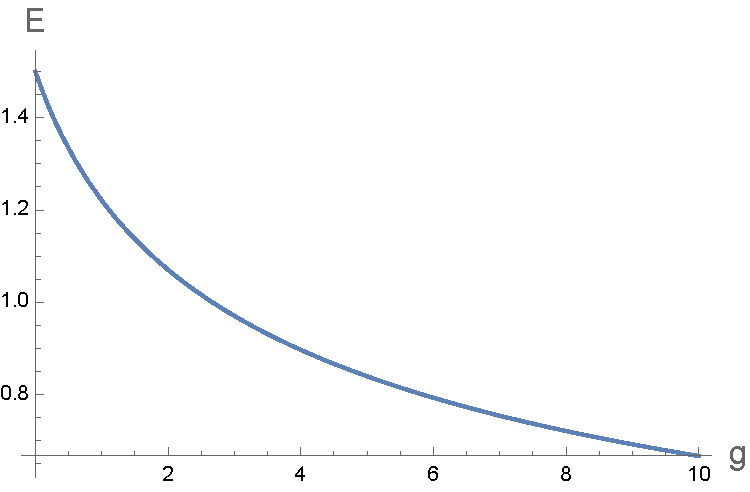
\includegraphics[width=0.7\columnwidth]{source_compendium/figures/2510_11766/ho4_energy_pert.pdf}
    \caption{The ground state energy of the anharmonic oscillator as a function of~$g$. This is based on the next-to-leading estimate in the perturbation theory in terms of~$g$. The quantum numbers, $n_r$ and~$l$, are set to vanish, so $\lambda=1/2$ under the Langer correction. Typically, the energy is damping monotonically with respect to the perturbation parameter~$g$.}
    \label{src:2510_11766:fig:ho4_energy_pert}
\end{figure}
Now, we define $Q=r^2 + \frac{g}{2}r^4 + \frac{\lambda^2}{r^2} - 2E$ and $Q^0 = \alpha^2 r^2 + \frac{\lambda^2}{r^2} - 2 E$, and so obtain
\begin{align}
    \mathcal{S}^0 &= \sqrt{r^2 + \frac{\lambda^2}{r^2} - 2 E} , \\
    \mathcal{S}^1 &= \frac{1}{2} \frac{\frac{g}{2} r^4}{\sqrt{r^2 + \frac{\lambda^2}{r^2} - 2 E}}, \qquad \dots,
\end{align}
and
\begin{align}
    \oint \rmd r\, \mathcal{S}^0 &= 2\rmi \pi \left(\frac{E}{\alpha} - \lambda\right) ,\\
    \oint \rmd r\, \mathcal{S}^1
    &= \pm \rmi \pi \frac{\alpha^2 - E g (1 - 2 \alpha^2)}{4 g \alpha^{3}} + O(g) .
\end{align}
Note that $\mathcal{S}^1$ is expanded in terms of $g$ before integrating. The fastest apparent convergence up to $O(g)$ gives 
\begin{align}
    \partial_\alpha\left[\frac{E}{\alpha} - \lambda \pm \frac{1}{2}\frac{\alpha^2 - E g (1 - 2 \alpha^2)}{4 g \alpha^{3}}\right] = 0 ,
    \label{src:2510_11766:eq:fac_condition_anharmonic}
\end{align}
and we obtain
\begin{align}
    \alpha^{(1)} = \pm\sqrt{\frac{3gE}{1 + 10gE}}, \qquad
    \pm\sqrt{\frac{3gE}{1 - 6gE}} ,
\end{align}
where the first and second solutions are for $+$ and for $-$, respectively, in Eq.~\eqref{src:2510_11766:eq:fac_condition_anharmonic}.
Hence, for instance $\alpha^{(1)} = \sqrt{\frac{3gE}{1 + 10gE}}$, we see
\begin{align}
    \frac{\sqrt{1 + 10gE}}{12 \sqrt{3E} g^{3/2}} + \frac{5 \sqrt{E} \sqrt{1 + 10gE}}{6 \sqrt{3g}} - \lambda &= 2n_r + 1
    \\
    \frac{(1+10 g E)^{3/2}}{\sqrt{E}} &= 12\sqrt{3}g^{3/2}(2n_r + 1 + \lambda) ,
    \label{src:2510_11766:eq:ho4_energy}
%    \\
%    \frac{(1+10 g E)^{3}}{E} &= [12\sqrt{3}g^{3/2}(2n_r + 1 + \lambda)]^2
%    \\
%    \frac{1+30gE+300g^2E^2+1000g^3E^3}{E} &= [12\sqrt{3}g^{3/2}(2n_r + 1 + \lambda)]^2
\end{align}
and depicted the ground state energy~$E$ with~$n_r=0$, $\lambda=1/2$ in Fig.~\ref{src:2510_11766:fig:ho4_energy}, which grows along~large $g$ typically.
There are some roots of the algebraic equations with regard to~$E$. Almost those are non-physical due to, e.g., negative energy. We here illustrate a more plausible result for $g>\frac{1}{6}\sqrt{\frac{5}{2}}$.
Of course, these are not results with such a high level of precision; even within the variational perturbation theory (with parameter $\delta$), the function of $g$ is expanded in powers of $g$, and we do not address the systematic issues of truncated fastest apparent convergence in any serious manner.
\begin{figure}[t]
    \centering
    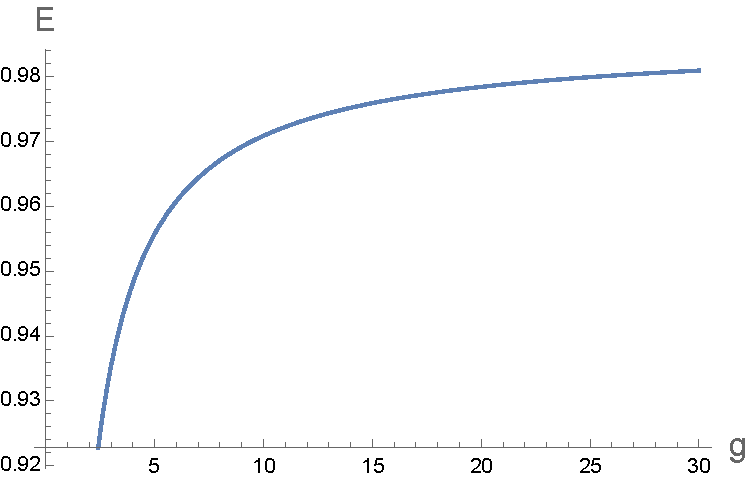
\includegraphics[width=0.7\columnwidth]{source_compendium/figures/2510_11766/ho4_energy.pdf}
    \caption{The ground state energy of the anharmonic oscillator as a function of~$g$. The derivation is given by the variational method with the fastest apparent condition up to subleading of~$g$, and the explicit function is given by~Eq.~\eqref{src:2510_11766:eq:ho4_energy}. The quantum numbers, $n_r$ and~$l$, are set to vanish, so $\lambda=1/2$ under the Langer correction. Typically, the energy is growing up monotonically with respect to~$g$.}
    \label{src:2510_11766:fig:ho4_energy}
\end{figure}
\subsection{Variations of Coulomb}\label{src:2510_11766:sec:cornell_yukawa}
In this calculation module, we consider the Cornell/Yukawa potential,
\begin{align}
    V_C(r) &= - \frac{\Tilde\alpha}{r} + \sigma r, &
    V_Y(r) &= - \frac{\rme^{-\mu r}}{r} ,
\end{align}
where the turning points are given by
\begin{align}
    a_C^\pm &= \frac{E}{2\sigma} \pm \sqrt{\frac{E^2}{4\sigma^2} + \frac{\Tilde\alpha}{\sigma}}, &
    a_Y^+ &= \frac{1}{\mu} W(-\mu/E) ,
\end{align}
respectively.
Here $W(z)$ is the Lambert W-function.
The Stokes structure of the Cornell potential is shown in Fig.~\ref{src:2510_11766:fig:stokes_cornell}. For the Yukawa potential, the Stokes structure is the same as for Coulomb potential in Fig.~\ref{src:2510_11766:fig:stokes_coulomb}.
%We set $Q=-\frac{\rme^{-\mu r}}{r}+\frac{\lambda^2}{r^2}-2E$ and $Q^0=-\frac{\alpha}{r}+\frac{\lambda^2}{r^2}-2E$.
%\begin{align}
%    \mathcal S^0 &= \sqrt{-\frac{\alpha}{r}+\frac{\lambda^2}{r^2}-2E},\\
%    \mathcal S^1 &= \frac{1}{2} \frac{\alpha-\rme^{-\mu r}}{r\sqrt{-\frac{\alpha}{r}+\frac{\lambda^2}{r^2}-2E}}
%\end{align}
%\begin{align}
%    \oint \mathcal S^0 &= 2\rmi \pi \frac{\alpha}{\sqrt{-2E}}
%    \\
%    \oint \mathcal S^1 &=
%\end{align}
\begin{figure}[t]
\centering
\begin{tikzpicture}[scale=0.8,transform shape]
    \draw[very thick] (0,0) -- (-3,0);
    \draw[very thick] (3,0) -- (6,0) node[right] {$-$};
    \draw[very thick] (3,0) arc(40:92.5:10) node[left] {$+$};
    \draw[very thick] (3,0) arc(-40:-92.5:10) node[left] {$+$};
    \draw[very thick] (-3,0) arc(40:60:10) node[left] {$+$};
    \draw[very thick] (-3,0) arc(-40:-60:10) node[left] {$+$};
    %
    \draw[very thick,blue,snake it] (0,0) -- (3,0);
    %
    \fill[white] (0,0) circle(3pt);
    \draw[ultra thick] (0,0) circle(3pt) node[below] {$0$};
    \fill (3,0) circle(3pt) node[below right] {\Large $a_C^+$};
    \fill (-3,0) circle(3pt) node[below right] {\Large $a_C^-$};
    %
    \draw[ultra thick,red,->] (6,1) -- (0,1) arc(90:270:1) -- (6,-1);
\end{tikzpicture}
\caption{Schematic Stokes graph for the Cornell potential.}
\label{src:2510_11766:fig:stokes_cornell}
\end{figure}
Again, we can find the same quantization condition
\begin{align}
    \cosh\left(\oint_0^{a^+} \rmd r\, \vsub{S}{odd}\right)
    + \cos(\pi(2l+1)) = 0 .
\end{align}
The next-to-leading order contributes as
\begin{align}
    \frac{1}{2\pi} \oint_0^{a_C^+} \rmd r\, S_{-1}
    &= \rmi \frac{\Tilde\alpha}{\sqrt{-2E}} -\frac{3 \rmi  \Tilde\alpha^2 \sigma }{8 \sqrt{2} (-E)^{5/2}} + O(\sigma^2), \\
    \frac{1}{2\pi} \oint_0^{a_Y^+} \rmd r\, S_{-1}
    &= \rmi \frac{1}{\sqrt{-2E}} -\frac{\rmi  \mu }{2 \sqrt{2} (-E)^{3/2}} + O(\mu^2) .
\end{align}
Figure~\ref{src:2510_11766:fig:CY_coulomb_energy} shows the ground state energies of the two potentials as functions of the corresponding parameters introduced to deform the Coulomb potential. The behavior in terms of $\sigma$ or $\mu$ is reasonable.
\begin{figure}[t]
    \centering
    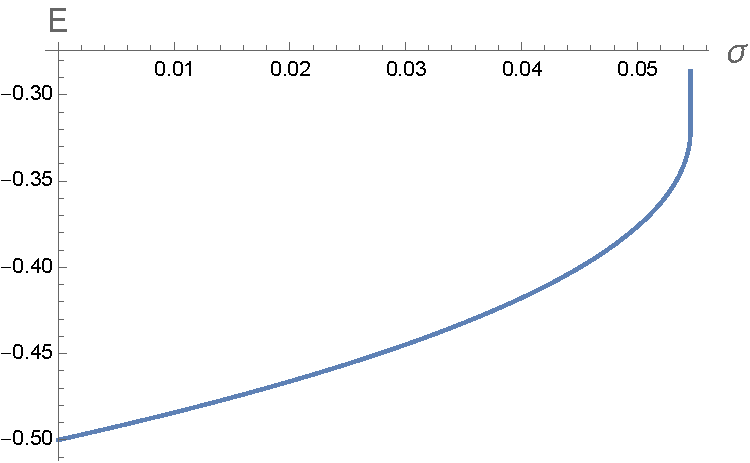
\includegraphics[width=0.45\columnwidth]{source_compendium/figures/2510_11766/cornell_energy.pdf}
    \hspace{1em}
    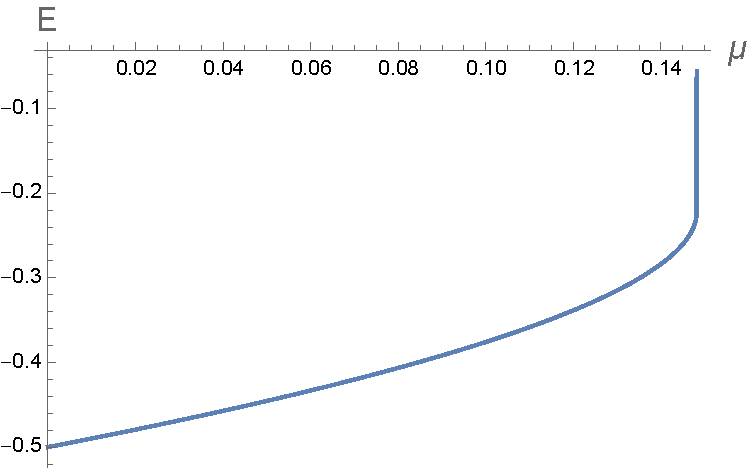
\includegraphics[width=0.45\columnwidth]{source_compendium/figures/2510_11766/yukawa_energy.pdf}
    \caption{The ground state energy of the variations of the Coulomb potential: \textbf{(Left)} Cornell potential with $\Tilde\alpha=1$ as a function of~$\sigma$, and \textbf{(Right)} Yukawa potential as a function of~$\mu$. The quantum numbers, $n_r$ and~$l$, are set to be zero. Typically, the energy is growing up monotonically with respect to the perturbation parameters, $\sigma$ and $\mu$.}
    \label{src:2510_11766:fig:CY_coulomb_energy}
\end{figure}
\subsection{Open-path and closed-cycle equivalence: a general statement}
\label{src:2510_11766:sec:open-closed}
Consider the radial Schr\"odinger equation
\begin{align}
\label{src:2510_11766:eq:radial}
    \left[- \frac{\hbar^2}{2}\frac{\rmd^2}{\rmd r^2} + V(r) + \frac{\hbar^2 (\ell+\tfrac12)^2}{2r^2} \right] u(r) = E\,u(r),    
\end{align}
where we have incorporated the Langer improvement $\ell(\ell+1)\to(\ell+\tfrac12)^2$.
Suppose that $V$ is meromorphic. We assume:
\begin{itemize}
\item[(A1)] $V$ extends analytically to a simply connected domain $\mathcal D\subset\mathbb C$ containing $[0,+\infty)$ and the Stokes graph relevant to the energy $E$.
\item[(A2)] $r=0$ is a \textit{regular} singular point of Eq.~\eqref{src:2510_11766:eq:radial}.
\item[(A3)] $E$ belongs to the discrete spectrum, so that a subdominant solution exists as $r\to+\infty$ in some Stokes sector.
\item[(A4)] The Borel sums of the exact-WKB objects used below exist in a fixed lateral direction $\theta$ not crossing a Stokes curve.
\end{itemize}
Let $\Gamma$ be a closed contour that goes from $+\infty$ to the vicinity of $r=0$ within a Stokes sector, encircles $r=0$ once counterclockwise on the same sheet, and returns to $+\infty$.
%We write
%\begin{align}
%    \mathcal W_\Gamma(E,\hbar):= \rme^{\oint_\Gamma \rmd r\,\vsub{S}{odd}(r;E,\hbar)}
%\end{align}
%for the (Borel-summed) Voros symbol along $\Gamma$, and $\mathcal S_\Gamma(E,\hbar)$ for the ordered product of Stokes multipliers encountered along $\Gamma$ (both are independent of local normalizations). We denote by $\vsub{\gamma}{mon}(E,\hbar)\in\mathbb R/\mathbb Z$ the \textit{monodromy phase} of a local Frobenius basis at $r=0$ after factoring out the geometric phase associated with~\eqref{src:2510_11766:eq:radial}.
\begin{proposition}[\textbf{Open-path $\Leftrightarrow$ Closed-cycle under A1--A4}]
For a given $E$, the following are equivalent:
\begin{description}
\item[(i)] \textbf{Open-path quantization:} There exists a nontrivial solution of Eq.~\eqref{src:2510_11766:eq:radial} which is subdominant as $r\to+\infty$ and \textit{regular} at $r=0$ (i.e. no logarithmic growth in the Frobenius expansion).
\item[(ii)] \textbf{Closed-cycle exact-WKB quantization:} The monodromy gathered along $\Gamma$ has a zero point, i.e.
\begin{align}
    \label{src:2510_11766:eq:closed-quantization}
    \cosh\left(\oint_\Gamma \rmd r\, \vsub{S}{odd}\right)
    + \cos(\pi\sqrt{1+4Q_2}) = 0 .
\end{align}
In other words, the monodromy phase in terms of~$\vsub{\gamma}{mon}$ has a unit with the ordered product of Stokes multipliers encountered along $\Gamma$.
%\begin{align}
%\label{src:2510_11766:eq:closed-quantization}
%    \mathcal W_\Gamma(E,\hbar)\,\mathcal S_\Gamma(E,\hbar)\,\rme^{2\pi \rmi \,\vsub{\gamma}{mon}(E,\hbar)}=1 .
%\end{align}
\end{description}
\end{proposition}
\subparagraph{Sketch of proof}
Fix a decaying solution $\psi_\infty$ at $+\infty$ (lateral Borel sum at angle $\theta$), and a local Frobenius basis $(\vsup{\psi}{reg}_0,\vsup{\psi}{sing}_0)$ at $r=0$, where $\vsup{\psi}{reg}_0$ and $\vsup{\psi}{sing}_0$ are the regular and singular solutions at the origin, respectively. Transport $\psi_\infty$ to the origin across Stokes curves, multiplying by the corresponding monodromy matrices (AKT connection). One obtains
\begin{align}
    \psi_\infty = \vsub{C}{reg}(E,\hbar)\,\vsup{\psi}{reg}_0 + \vsub{C}{sing}(E,\hbar)\,\vsup{\psi}{sing}_0,
\end{align}
with connection coefficients expressed through Voros and Stokes multipliers. Condition (i) in Proposition holds iff $\vsub{C}{sing}(E,\hbar)=0$. Now close the path by a small counterclockwise loop around $r=0$ and return to $+\infty$; the net transport along this closed contour amounts to multiplication by Stokes multipliers and~$\rme^{2\pi \rmi \vsub{\gamma}{mon}}$ in a suitable basis. Triangularity of the local monodromy at a regular singularity and Wronskian conservation (i.e., the condition so that the coefficient of dominant solution on the right hand side should vanish as usual) imply that $\vsub{C}{sing}=0$ iff the closed monodromy has a zero point (monodromy unit), which is precisely Eq.~\eqref{src:2510_11766:eq:closed-quantization}. Independence of Eq.~\eqref{src:2510_11766:eq:closed-quantization} from local normalizations follows from the standard arbitrariness of choosing Stokes data.
\hfill$\square$
For the 3D harmonic oscillator and for the Coulomb problem, one can choose $\Gamma$ such that $\vsub{\gamma}{mon}=0$; then the second term on the left-hand side in Eq.~\eqref{src:2510_11766:eq:closed-quantization} is moved to the right-hand side (with the Langer improvement).
The statement presumes regularity at the origin and excludes irregular singular points and energies for which Stokes curve accumulate around $r=0$.
If $V$ has additional singularities or branch points in $\mathcal D$, the contour $\Gamma$ must be chosen to avoid them (see Sec.~\ref{src:2510_11766:sec:anharmonic}); otherwise extra factors contribute.
The Bohr--Sommerfeld quantization is now given in the form as
\begin{equation}
\label{src:2510_11766:eq:QC-practical}
\frac{1}{2\pi\hbar}\oint_\Gamma \vsub{p}{eff}(r;E)\dd r
\;+\; \Phi_\Gamma(E,\hbar) \;+\; \vsub{\gamma}{mon}(E,\hbar)\;\in\; \mathbb Z,
\end{equation}
where
$\vsub{p}{eff}(r;E):=\sqrt{2m\,(E-\vsub{V}{eff}(r))}$ with $\vsub{V}{eff}(r):=V(r)+\hbar^2(\ell+\tfrac12)^2/(2r^2)$, and $\Phi_\Gamma$ collects all higher-order WKB/Voros corrections and Stokes contributions along $\Gamma$.

\subsection*{Laboratory checkpoint}
Before moving to the next stage, perform the following checks without copying
the displayed final answer.
\begin{enumerate}
  \item Derive the Langer term directly from the exponential coordinate map rather than inserting it as a remembered replacement rule.
  \item Recover the oscillator and Coulomb quantization conditions from both open-path matching and closed-cycle monodromy.
  \item Vary the auxiliary deformation or optimization parameter and impose monodromy independence before treating the Cornell or Yukawa case.
\end{enumerate}
